\documentclass[french,bookmarks,aspectratio=43]{beamer}

\usepackage{tikz}
\usepackage{siunitx}
\usepackage{svg}
\usepackage{nicematrix}
\usepackage{booktabs}
\usetikzlibrary{angles, quotes, graphdrawing.trees, tikzmark, decorations.markings,decorations.pathreplacing, positioning, 3d, shapes.misc, shapes.geometric, automata, arrows,calc,positioning}
\makeatletter

\newcommand*\bigcdot{\mathpalette\bigcdot@{2}}
\newcommand*\bigcdot@[2]{\mathbin{\vcenter{\hbox{\scalebox{#2}{$\m@th#1\bullet$}}}}}

\AtBeginSection[]{\frame{\sectionpage}}
%\AtBeginSubsection[]{\frame{\subsectionpage}}

\newcommand{\my@bigsize}{9}
\newcommand{\my@medsize}{7}
\newcommand{\my@smallsize}{5}

\newlength{\my@tempsize}

\newcounter{my@sectnum}

\newcommand{\my@lastdigit}[1]{%
  \loop\ifnum\value{#1}>9\addtocounter{#1}{-10}\repeat
  \arabic{#1}%
}

\newcommand\my@fixedbox[2]{%
  \makebox[#1]{\rule[-1ex]{0pt}{3.25ex}#2}%
}

\newcommand\my@colorbox[3]{%
  {\setlength{\fboxsep}{0pt}\colorbox{#1}{\my@fixedbox{#2}{#3}}}%
}

\def\my@temptext{}

\newcommand{\my@navbox}[1][]{%
  \if\relax\detokenize{#1}\relax
    \def\my@tempbox{\my@fixedbox}%
  \else
    \def\my@tempbox{\my@colorbox{#1}}%
  \fi
  \ifx\my@box\my@bigbox
    \def\my@temptext{\my@lastdigit{my@sectnum}}%
  \fi
  \ifx\my@box\my@medbox
    \def\my@temptext{$\diamond$}%
  \fi
  \ifx\my@box\my@smallbox
    \def\my@temptext{$-$}%
  \fi
  \my@tempbox{\my@tempsize}{\my@temptext}%
}

\defbeamertemplate{navigation box}{home}{%
  \setlength{\my@tempsize}{\my@box@size pt}%
  \my@colorbox{main3!20}{\my@tempsize}{$\equiv$}%
}

\defbeamertemplate{navigation box}{done}{%
  \setlength{\my@tempsize}{\my@box@size pt}%
  \my@navbox[main3!20]%
}

\defbeamertemplate{navigation box}{todo}{%
  \setlength{\my@tempsize}{\my@box@size pt}%
  \my@navbox
}

\newcommand{\my@bigbox}{\global\let\my@box@size=\my@bigsize\usebeamertemplate{navigation box}}
\newcommand{\my@medbox}{\global\let\my@box@size=\my@medsize\usebeamertemplate{navigation box}}
\newcommand{\my@smallbox}{\global\let\my@box@size=\my@smallsize\usebeamertemplate{navigation box}}

\renewcommand{\sectionentry}[5]{\global\let\my@box=\my@bigbox\setcounter{my@sectnum}{#1}}
\renewcommand{\beamer@subsectionentry}[5]{\global\let\my@box=\my@medbox}

\renewcommand{\slideentry}[6]{%
  \def\my@temp@i{1/1}%
  \def\my@temp@ii{#4}%
  \ifx\my@temp@i\my@temp@ii % title page
    \setbeamertemplate{navigation box}[home]%
  \else
    \setbeamertemplate{navigation box}[done]%
  \fi
  \ifnum\c@section<#1%
    \setbeamertemplate{navigation box}[todo]%
  \else
    \ifnum\c@section=#1\ifnum\c@subsection<#2%
      \setbeamertemplate{navigation box}[todo]%
    \else
      \ifnum\c@subsection=#2\ifnum\c@subsectionslide<#3%
        \setbeamertemplate{navigation box}[todo]%
      \fi\fi
    \fi\fi
  \fi
  \ifx\my@temp@i\my@temp@ii % title page
    \beamer@link(#4){\my@bigbox}%
  \else
    \beamer@link(#4){\my@box}%
  \fi
  \global\let\my@box=\my@smallbox
}

\defbeamertemplate{footline}{progress}
{%
  {\color{main3}\hrule}\hbox{%
  \begin{beamercolorbox}[wd=.8\paperwidth,ht=2.25ex,dp=1ex,left]{footline}%
    \kern2em\dohead
  \end{beamercolorbox}%
  \begin{beamercolorbox}[wd=.2\paperwidth,ht=2.25ex,dp=1ex,right]{footline}%
  \insertframenumber{}/\inserttotalframenumber\kern2em
  \end{beamercolorbox}%
  }%
}

\setbeamertemplate{navigation symbols}{}
\setbeamertemplate{footline}[progress]

\makeatother

\usetheme{default}
\usecolortheme{seahorse}

\usepackage{lmodern}
\usepackage{babel}
\usepackage[T1]{fontenc}
\usepackage{stmaryrd}

\usepackage{xparse}
\usepackage[most,breakable,listings]{tcolorbox}

\usefonttheme[onlymath]{serif}

%\newfontfamily{\EBGaramond}{EBGaramond}[RawFeature={+clig,+liga,+cv11,+cv90,+calt,+ccmp,+swsh},Ligatures=TeX]

%\defaultfontfeatures{RawFeature={+hlig,+clig,+liga,+cv11,+cv90,+calt,+ccmp,+swsh},Ligatures=TeX} %+dlig ?


\definecolor{main1} {RGB}{8, 127, 196}

\definecolor{main1comp} {RGB}{218, 65, 103}
\definecolor{main1comp2} {RGB}{119, 186, 153}
\definecolor{main1white} {RGB}{121, 129, 134}
\definecolor{main1white2} {RGB}{204, 204, 204}
\definecolor{main2} {RGB}{64, 115, 192}
\definecolor{main3} {RGB}{96, 102, 183}
\definecolor{main4} {RGB}{120, 86, 169}
\definecolor{main5} {RGB}{139, 69, 149}
\definecolor{main6} {RGB}{152, 51, 126}
\definecolor{main7} {RGB}{158, 30, 100}
\definecolor{main8} {RGB}{159, 4, 72}
\definecolor{main9} {RGB}{153, 0, 44}
\definecolor{main10} {RGB}{142, 1, 15}
\definecolor{main10comp} {RGB}{250, 126, 97}
\definecolor{main10comp2} {RGB}{63, 136, 197}

\definecolor{main20} {RGB}{7, 163, 106}
\definecolor{main21} {RGB}{184, 0, 0}

\definecolor{ocamlColor} {RGB}{242, 130, 17}

\setbeamercolor{titlelike}{parent=structure,bg=main3,fg=white}

\setbeamertemplate{sections/subsections in toc}[square]

\DeclareDocumentCommand\declarecours{mmmm}{
    \newtcbtheorem[]{AUX_#1}{\vphantom{Ép}#2}{
        breakable,
        enhanced,
        top = 5mm,
        before skip balanced = \tcboxedtitleheight/3,
        separator sign={\quad},
        %separator sign={\ \ding{228}},
        %if odd page={
            attach boxed title to top left={
                yshift=-\tcboxedtitleheight/2,
                xshift=-2mm
            },
            boxed title style={
                frame code={
                    \path[fill = #4!90]
                    %left color=#4!90!gray!90, right color=#4!85!gray!75] 
                        (frame.north west) -- 
                        (frame.north east) -- 
                        (frame.south east) -- 
                        (frame.south west) -- 
                        cycle;
                },
                interior engine=empty,
            },
        %}{
        %    attach boxed title to top right={
        %        yshift=-\tcboxedtitleheight/3,
        %        xshift=2mm
        %    },
        %    boxed title style={
        %        frame code={
        %            \path[right color=#4!90!gray!90, left color=#4!85!gray!75]
        %                (frame.north west) -- 
        %                (frame.north east) -- 
        %                (frame.south east) -- 
        %                (frame.south west) -- 
        %                cycle;
        %        },
        %        interior engine=empty,
        %    }
        %},
        fonttitle           = \sffamily,
        %borderline west     = {.5pt}{0pt}{#4!85!gray!50},
        %borderline north    = {\tcboxedtitleheight/3}{-\tcboxedtitleheight/3}{#4!85!gray!50},
        %borderline east     = {.5pt}{0pt}{#4!85!gray!50},
        %borderline south    = {.5pt}{0pt}{#4!85!gray!50},
        interior style      = {
            fill            = #4!10
            %left color      = #4!100!gray!8,
            %middle color    = #4!75!gray!7,
            %right color     = #4!50!gray!6
        },
        sharp corners   = downhill,
        arc             = 0 cm,
        boxrule         = 0pt,
        frame hidden%,
        %drop fuzzy shadow=#4!3
    }{#3}
    \newenvironment{#1}[2]{
        \begingroup
        \renewcommand{\bf}[1]{{\color{#4}\textbf{####1}}}
        \newcommand{\hg}[1]{\begingroup\color{#4}{####1}\endgroup}
        \newcommand{\hgu}[1]{\begingroup\color{#4}\underline{####1}\endgroup}
        \newcommand{\hguo}[1]{\begingroup\colorlet{cb@savedHGUO}{.}\color{#4}\underline{\color{cb@savedHGUO}####1}\endgroup}
        \newcommand{\boxedcol}[1]{\begingroup\colorlet{cb@savedBOX}{.}\color{#4}\boxed{\color{cb@savedBOX}####1}\endgroup}
        \begin{AUX_#1*}{##1}{##2}
    }{
        \end{AUX_#1*}
        \endgroup
        \global\def\nproofcolor{#4}
    }
    \expandafter\NewDocumentCommand\csname #3ref\endcsname{m}{\textsc{\smartref{#3:##1} }}
}

\declarecours{bdefinition}{Définition}{def}{main1}
\declarecours{bproperty}{Propriété}{prop}{main3}
\declarecours{blemma}{Lemme}{lem}{main6}
\declarecours{btheorem}{Théorème}{th}{main10}
\declarecours{bcorrolary}{Corollaire}{cor}{main9}

\DeclareDocumentCommand\declarecoursalt{mmmm}{
    \newtcbtheorem[]{AUX_#1}{#2}{
        theorem name,
        breakable,
        enhanced,
        top = 3mm,
        separator sign={\quad},
        attach boxed title to top center={
            yshift=-\tcboxedtitleheight/2,
        },
        colframe            = {#4},
        borderline west     = {.5pt}{0pt}{#4},
        borderline north    = {.5pt}{0pt}{#4},
        borderline east     = {.5pt}{0pt}{#4},
        borderline south    = {.5pt}{0pt}{#4},
        colback             = #4!1,
        fonttitle           = \sffamily,
        sharp corners       = downhill,
        arc                 = 0 cm,
        boxrule             = 0pt,
        frame hidden,
        %drop fuzzy shadow=#4!10!white,
        boxed title style={
        frame code={
            \path[left color=#4!95!gray!90,right color=#4!95!gray!90, middle color=#4!70!gray!90, fill=white] 
                    ([xshift=-2mm]frame.north west) -- 
                    ([xshift=2mm]frame.north east) -- 
                    ([xshift=2mm]frame.south east) -- 
                    ([xshift=-2mm]frame.south west) -- 
                    cycle;
        },
        interior engine=empty,
        }
    }{#3}
    \newenvironment{#1}[2]{
        \begingroup
        \renewcommand{\bf}[1]{{\color{#4}\textbf{####1}}}
        \newcommand{\hg}[1]{\begingroup\color{#4}{####1}\endgroup}
        \newcommand{\hgu}[1]{\begingroup\color{#4}\underline{####1}\endgroup}
        \newcommand{\hguo}[1]{\begingroup\colorlet{cb@savedHGUO}{.}\color{#4}\underline{\color{cb@savedHGUO}####1}\endgroup}
        \newcommand{\boxedcol}[1]{\begingroup\colorlet{cb@savedBOX}{.}\color{#4}\boxed{\color{cb@savedBOX}####1}\endgroup}
        \begin{AUX_#1*}{##1}{##2}
    }{
        \end{AUX_#1*}
        \endgroup
    }
    \expandafter\NewDocumentCommand\csname #3ref\endcsname{m}{\textsc{\smartref{#3:##1}}}
}

\declarecoursalt{bexample}{Exemple}{example}{main2}
\declarecoursalt{bexercise}{Exercice}{exo}{main20}
\declarecours{bexotd}{Exercice}{exotd}{main20}
\declarecoursalt{bwarning}{Avertissement}{warn}{main21}

\declarecoursalt{bform}{}{form}{black}


\newenvironment{psse}{
    \begin{enumerate}[label=\textrm{\rmfamily\itshape(\roman*)}]
}{
    \end{enumerate}
}

\newcommand{\pssenum}[1]{\textrm{\rmfamily\itshape(#1)}}

\newenvironment{expcom}{
    \begingroup
    \begin{tcolorbox}[
        breakable,
        enhanced,
        interior style      = {
            left color      = main1white2!65!gray!8,
            middle color    = main1white2!50!gray!7,
            right color     = main1white2!35!gray!6
        },
        %borderline north    = {.3pt}{0pt}{main1white!10},
        %borderline south    = {.3pt}{0pt}{main1white!10},
        %borderline west     = {2pt}{0pt}{colexp!85!gray!50},
        sharp corners       = downhill,
        frame hidden,
        arc                 = 0 cm,
        boxrule             = 0 cm,
        nobeforeSTYLE,
        noafterSTYLE,
        overlay={\begin{tcbclipinterior}
            \path[top color=colexp!85!gray!45, middle color=colexp!85!gray!55, bottom color=colexp!85!gray!55, fill=white] 
                    (interior.north west) -- 
                    ([xshift=2pt]interior.north west) -- 
                    ([xshift=2pt]interior.south west) -- 
                    (interior.south west) -- 
                    cycle;
                    
        \end{tcbclipinterior}}
    ]
        \begin{proofpure}[Compte-rendu]
}{
        \end{proofpure}
    \end{tcolorbox}
    \endgroup
}

\newenvironment{notation}{
    \begingroup
    \begin{tcolorbox}[
        breakable,
        enhanced,
        interior style      = {
            left color      = main1white2!65!gray!8,
            middle color    = main1white2!50!gray!7,
            right color     = main1white2!35!gray!6
        },
        sharp corners       = downhill,
        frame hidden,
        arc                 = 0 cm,
        boxrule             = 0 cm,
        nobeforeSTYLE,
        noafterSTYLE,
        overlay={\begin{tcbclipinterior}
            \path[top color=main1!95!gray!90, bottom color=main1!90!gray!70, fill=white] 
                    (interior.north west) -- 
                    ([xshift=2pt]interior.north west) -- 
                    ([xshift=2pt]interior.south west) -- 
                    (interior.south west) -- 
                    cycle;
                    
        \end{tcbclipinterior}}
    ]
        \small\textbf{\color{main1!95!gray!90} \textsf{(Notation)}}\newcommand{\hg}[1]{\begingroup\color{main1!95!gray!90}{##1}\endgroup}
}{
    \end{tcolorbox}
    \endgroup
}

\newenvironment{hpnote}{
    \begingroup
    \begin{tcolorbox}[
        breakable,
        enhanced,
        interior style      = {
            left color      = main1white2!65!gray!8,
            middle color    = main1white2!50!gray!7,
            right color     = main1white2!35!gray!6
        },
        sharp corners       = downhill,
        frame hidden,
        arc                 = 0 cm,
        boxrule             = 0 cm,
        nobeforeSTYLE,
        noafterSTYLE,
        overlay={\begin{tcbclipinterior}
            \path[top color=main1!85!gray!70, bottom color=main1!85!gray!50, fill=white] 
                    (interior.north west) -- 
                    ([xshift=2pt]interior.north west) -- 
                    ([xshift=2pt]interior.south west) -- 
                    (interior.south west) -- 
                    cycle;
                    
        \end{tcbclipinterior}}
    ]
        \textbf{\color{main1!95!gray!90} \textsf{(HP)}}
}{
        
    \end{tcolorbox}
    \endgroup
}
    
\newcommand{\demo}[1]{
    \begin{tcolorbox}[
        breakable,
        enhanced,
        interior style      = {
            left color      = main3!66!gray!13,
            middle color    = main3!33!gray!9,
            right color     = main3!0!gray!5
        },
        borderline north    = {.3pt}{0pt}{main3!5},
        borderline south    = {.3pt}{0pt}{main3!5},
        borderline west     = {1.5pt}{0pt}{main3!30},
        sharp corners       = downhill,
        arc                 = 0 cm,
        boxrule             = 0 cm,
    ]

        \begin{proof}
            #1
        \end{proof}
    \end{tcolorbox}
}

\newcommand{\demoth}[1]{
    \begin{tcolorbox}[
        breakable,
        enhanced,
        interior style      = {
            left color      = main10!66!gray!13,
            middle color    = main10!33!gray!9,
            right color     = main10!0!gray!5
        },
        borderline north    = {.3pt}{0pt}{main10!5},
        borderline south    = {.3pt}{0pt}{main10!5},
        borderline west     = {1.5pt}{0pt}{main10!30},
        sharp corners       = downhill,
        arc                 = 0 cm,
        boxrule             = 0 cm
    ]

        \begin{proof}
            #1
        \end{proof}
    \end{tcolorbox}
}

\newcommand{\demolm}[1]{
    \begin{tcolorbox}[
        breakable,
        enhanced,
        interior style      = {
            left color      = main6!66!gray!13,
            middle color    = main6!33!gray!9,
            right color     = main6!0!gray!5
        },
        borderline north    = {.3pt}{0pt}{main6!5},
        borderline south    = {.3pt}{0pt}{main6!5},
        borderline west     = {1.5pt}{0pt}{main6!30},
        sharp corners       = downhill,
        arc                 = 0 cm,
        boxrule             = 0 cm
    ]

        \begin{proof}
            #1
        \end{proof}
    \end{tcolorbox}
}
    
\makeatletter
\newcommand{\exlower}{%
  \begin{tikzpicture}
  \path[use as bounding box] (0,0) -- (\linewidth,0);
  \draw[color=main2, dash dot]
        (0-\kvtcb@leftlower-\kvtcb@boxsep,0) --
        (\linewidth+\kvtcb@rightlower+\kvtcb@boxsep,0);
  \end{tikzpicture}%
  }
\makeatother

\DeclareDocumentCommand\suite{m}{{\left(#1\right)_{n \in \bdN}}} 
\DeclareDocumentCommand\suiteZ{m}{{\left(#1\right)_{n \in \bdN^*}}}

\DeclareDocumentCommand\serie{}{\textstyle{\sum\limits_{n \in \bdN}}}
\newcommand{\bdRp}{\mathbb{R}_+^*}
%note : bien mettre avant ExplSyntaxOn

\DeclareDocumentCommand\guill{m}{\og #1\fg{}}

\makeatletter
\newcommand{\kmath}[1][0.65]{%
  \mathpalette\@kmath{#1}%
}
\newcommand*{\@kmath}[2]{%
  \scalebox{#2}[#2]{$#1\mathbf{\itshape k}\m@th$}%
}
\makeatother

\newtcblisting{C}{
    enhanced, breakable,
    attach boxed title to top right={yshift=-\tcboxedtitleheight},
    interior style = {
        left color = main1!12,
        right color = main1!5
    },
    boxed title style = {
        frame code = {
            \path[left color=ocamlColor, right color=ocamlColor!80] 
                (frame.north west)++(-5pt,0) -- 
                (frame.north east) -- 
                (frame.south east) -- 
                (frame.south west) -- 
                cycle;
        },
        interior engine=empty,
    },
    sharp corners = downhill,
    arc = 0 cm,
    title = {\sffamily C},
    boxrule = 0 pt,
    listing only,
    %nobeforeafter,
    %after=\par\nointerlineskip,
    overlay = {
        \begin{tcbclipinterior}
            \fill[main1!30] (frame.south west) rectangle ([xshift=6mm]frame.north west);
        \end{tcbclipinterior}
    },
    listing options = {
        firstnumber=last,
        language = C,
        basicstyle=\footnotesize\ttfamily,
        numbers=left,
        numbersep=3.3mm,
        xleftmargin=3mm,
        numberstyle={\small\sffamily\color{main1!50!black}},
        aboveskip=\smallskipamount, 
        belowskip=\smallskipamount,
        emph={uint8_t, NULL,return,printf,unsigned,long,difftime},
        emphstyle={\bfseries\color{ocamlColor}},
        classoffset=1,
        morekeywords={>,<,=,&,|,^,[,],&,(,)},
        otherkeywords={>,<,=,&,|,^,[,],&,(,)},
        keywordstyle={\bfseries\color{main3}},
        classoffset=0,
    }
}

\newtcblisting{bash}{
    enhanced,
    attach boxed title to top right={yshift=-\tcboxedtitleheight},
    interior style = {
        left color = main1!12,
        right color = main1!5
    },
    boxed title style = {
        frame code = {
            \path[left color=ocamlColor, right color=ocamlColor!80] 
                (frame.north west)++(-5pt,0) -- 
                (frame.north east) -- 
                (frame.south east) -- 
                (frame.south west) -- 
                cycle;
        },
        interior engine=empty,
    },
    sharp corners = downhill,
    arc = 0 cm,
    title = {\sffamily Bash},
    boxrule = 0 pt,
    listing only,
    %nobeforeafter,
    %after=\par\nointerlineskip,
    overlay = {
        \begin{tcbclipinterior}
            \fill[main1!30] (frame.south west) rectangle ([xshift=6mm]frame.north west);
        \end{tcbclipinterior}
    },
    listing options = {
        style = tcblatex,
        language = bash,
        numbersep=3.3mm,
        xleftmargin=3mm,
        numberstyle={\small\sffamily\color{main1!50!black}},
        aboveskip=\smallskipamount, 
        belowskip=\smallskipamount,
    }
}

\lstnewenvironment{outputlog}{
    \lstset{
        tabsize=2,
        breaklines,
        basicstyle=\tiny\ttfamily,
        frame=leftline
    }
}{}


\ExplSyntaxOn

\DeclareDocumentCommand\funlv{mg}{
  \qopname\relax o{#1}
  \IfNoValueTF{#2}{}{\p{#2}}
}

\DeclareDocumentCommand\floor{m}{\left\lfloor#1\right\rfloor}


\DeclareDocumentCommand\funlvi{m}{
    \expandafter\DeclareDocumentCommand\expandafter{\csname #1\endcsname}{g}{\funlv{#1}{##1}}
}


\DeclareDocumentCommand\funlfv{mg}{
    \mathfrak{#1}
    \IfNoValueTF{#2}{}{\left(#2\right)}
}



\DeclareDocumentCommand\asymp{g}{%
    \IfNoValueTF{#1}{\sim}{\underset{#1}{\sim}}
}

\DeclareDocumentCommand\eq{g}{
    \IfNoValueTF{#1}{=}{\underset{#1}{=}}
}

%TODO: OPTIMISER EN CAS DUN SEUL ARG
\DeclareDocumentCommand\o{gg}{
    \IfNoValueTF{#1}{\bco}{\underset{#1}{\bco}}
    \IfNoValueTF{#2}{}{\p{#2}}
}

\DeclareDocumentCommand\O{gg}{
    \IfNoValueTF{#1}{\bcO}{\underset{#1}{\bcO}}
    \IfNoValueTF{#2}{}{\p{#2}}
}

\DeclareDocumentCommand\lima{g}{
    \IfNoValueTF{#1}{\xrightarrow[]{}}{\xrightarrow[#1]{}}
}

\DeclareDocumentCommand\rleq{}{\preccurlyeq}

\newcommand{\transp}{^{\!\mathsf{T}}}
\DeclareDocumentCommand\mtrans{m}{\,{}^\mathsf{t}\!#1}
\newcommand{\ii}{\mathrm{i\mkern1mu}}
\newcommand{\jj}{\mathrm{j\mkern1mu}}

\DeclareDocumentCommand\phyavg{m}{\left\langle#1\right\rangle}

\DeclareDocumentCommand\vec{m}{\overrightarrow{#1}}
\DeclareDocumentCommand\sfrac{mm}{\nicefrac{#1}{#2}}
\DeclareDocumentCommand\itb{}{\item[\bullet]}
\DeclareDocumentCommand\itob{}{\item[\circ]}
\DeclareDocumentCommand\itt{}{\item[\triangleright]}
\DeclareDocumentCommand\itast{}{\item[\ast]}
\DeclareDocumentCommand\its{m}{\item[\ding{#1}]}
\DeclareDocumentCommand\ithand{}{\its{43}}
\DeclareDocumentCommand\itstar{}{\its{73}}
\DeclareDocumentCommand\itvarstar{}{\its{72}}
\DeclareDocumentCommand\itarr{}{\its{226}}
\DeclareDocumentCommand\itvararr{}{\its{227}}
\DeclareDocumentCommand\itbox{}{\its{113}}
\DeclareDocumentCommand\itvarbox{}{\its{114}}
\DeclareDocumentCommand\cc{mmm}{\mathcal{C}^{#1}\left({#2},{#3}\right)}

%===============================
% Commandes pour les complexes
%===============================

\DeclareDocumentCommand\Bernoulli{}{\textsc{Bernoulli}}
\newcommand{\Pascal}{\textsc{Pascal}}
\newcommand{\Newton}{\textsc{Newton}}
\newcommand{\Euler}{\textsc{Euler}}

\DeclareDocumentCommand\Re{g}{\funlfv{Re}{#1}}
\DeclareDocumentCommand\Im{g}{\funlfv{Im}{#1}}
\DeclareDocumentCommand{\mod}{m}{\left\lvert#1\right\rvert}
\DeclareDocumentCommand{\norm}{m}{\left\lVert#1\right\rVert}
    
\DeclareDocumentCommand{\tnorm}{m}{{\left\vert\kern-0.25ex\left\vert\kern-0.25ex\left\vert #1 
    \right\vert\kern-0.25ex\right\vert\kern-0.25ex\right\vert}}

\DeclareDocumentCommand{\indication}{m}{{\footnotesize\rmfamily Indication :} \ {\footnotesize\emph{#1}}}
\DeclareDocumentCommand{\indef}{m}{\textit{\color{main1}#1}}
\DeclareDocumentCommand{\ens}{m}{\left\{#1\right\}}

\DeclareDocumentCommand{\dep}{m}{\left.#1\right\vert}

\DeclareDocumentCommand{\enstq}{}{\;\middle\vert\;}
\DeclareDocumentCommand{\benstq}{}{\;\vphantom{\dfrac{}{}}\middle\vert\;}

\DeclareDocumentCommand{\intc}{m}{\left[#1\right]}
\DeclareDocumentCommand{\iint}{m}{\left\llbracket#1\right\rrbracket}

\DeclareDocumentCommand{\into}{m}{\left]#1\right[}
\DeclareDocumentCommand{\iinto}{m}{\left\rrbracket#1\right\llbracket}

\DeclareDocumentCommand{\intor}{m}{\left[#1\right[}
\DeclareDocumentCommand{\iintor}{m}{\left\llbracket#1\right\llbracket}

\DeclareDocumentCommand{\intol}{m}{\left]#1\right]}
\DeclareDocumentCommand{\iintol}{m}{\left\rrbracket#1\right\rrbracket}

\DeclareDocumentCommand{\p}{m}{\!\left(#1\right)}


\DeclareDocumentCommand\arg{g}{\funlv{arg}{#1}}
\DeclareDocumentCommand{\expc}{m}{e^{i#1}}

\DeclareFontFamily{U}{mathc}{}
\DeclareFontShape{U}{mathc}{m}{it}%
{<->s*[1.03] mathc10}{}

\DeclareMathAlphabet{\mathcal}{U}{mathc}{m}{it}

%=====================================================%
%                                                     %
%   Commandes pour les lettres en "blackboard bold"   %
%  =-=-=-=-=-=-=-=-=-=-=-=-=-=-=-=-=-=-=-=-=-=-=-=-=  %
%                                                     %
%   Chaque "\bd[*]" où [*] est une lettre majuscule   %
%   est un alias à \mathbb{[*]}. On l'utilise géné-   %
%   ralement pour désigner les ensembles : N, Z, Q,   %
%   R pour les entiers, rationnels, réels, ...        %
%   La fonte de \mathbb utilisé ici est celle de la   %
%   distribution par défaut (LuaLaTeX est utilisé).   %
%                                                     %
%   Est aussi présente la commande \bdOne, laquelle   %
%   est un alias à \mathbbm{1}, et permet d'obtenir   %
%   le chiffre "1" en police "blackboard bold", qui   %
%   est utilisé pour désigner une fonction indica-    %
%   trice d'un ensemble.                              %
%   La fonte est importée par le package "bbm", qui   %
%   crée également la commande \mathbbm. Le chiffre   %
%   "1" n'est en effet pas disponible dans la fonte   %
%   par défaut de la distribution.                    %
%=====================================================%


\newcommand{\bdOne}{\mathbbm{1}}

\newcommand{\bdA}{\mathbb{A}}
\newcommand{\bdB}{\mathbb{B}}
\newcommand{\bdC}{\mathbb{C}}
\newcommand{\bdD}{\mathbb{D}}
\newcommand{\bdE}{\mathbb{E}}
\newcommand{\bdF}{\mathbb{F}}
\newcommand{\bdG}{\mathbb{G}}
\newcommand{\bdH}{\mathbb{H}}
\newcommand{\bdI}{\mathbb{I}}
\newcommand{\bdJ}{\mathbb{J}}
\newcommand{\bdK}{\mathbb{K}}
\newcommand{\bdL}{\mathbb{L}}
\newcommand{\bdM}{\mathbb{M}}
\newcommand{\bdN}{\mathbb{N}}
\newcommand{\bdO}{\mathbb{O}}
\newcommand{\bdP}{\mathbb{P}}
\newcommand{\bdQ}{\mathbb{Q}}
\newcommand{\bdR}{\mathbb{R}}
\newcommand{\bdS}{\mathbb{S}}
\newcommand{\bdT}{\mathbb{T}}
\newcommand{\bdU}{\mathbb{U}}
\newcommand{\bdV}{\mathbb{V}}
\newcommand{\bdW}{\mathbb{W}}
\newcommand{\bdX}{\mathbb{X}}
\newcommand{\bdY}{\mathbb{Y}}
\newcommand{\bdZ}{\mathbb{Z}}


\newcommand{\bcA}{\mathcal{A}}
\newcommand{\bcB}{\mathcal{B}}
\newcommand{\bcC}{\mathcal{C}}
\newcommand{\bcD}{\mathcal{D}}
\newcommand{\bcE}{\mathcal{E}}
\newcommand{\bcF}{\mathcal{F}}
\newcommand{\bcG}{\mathcal{G}}
\newcommand{\bcH}{\mathcal{H}}
\newcommand{\bcI}{\mathcal{I}}
\newcommand{\bcJ}{\mathcal{J}}
\newcommand{\bcK}{\mathcal{K}}
\newcommand{\bcL}{\mathcal{L}}
\newcommand{\bcM}{\mathcal{M}}
\newcommand{\bcN}{\mathcal{N}}
\newcommand{\bcO}{\mathcal{O}}
\newcommand{\bcP}{\mathcal{P}}
\newcommand{\bcQ}{\mathcal{Q}}
\newcommand{\bcR}{\mathcal{R}}
\newcommand{\bcS}{\mathcal{S}}
\newcommand{\bcT}{\mathcal{T}}
\newcommand{\bcU}{\mathcal{U}}
\newcommand{\bcV}{\mathcal{V}}
\newcommand{\bcW}{\mathcal{W}}
\newcommand{\bcX}{\mathcal{X}}
\newcommand{\bcY}{\mathcal{Y}}
\newcommand{\bcZ}{\mathcal{Z}}

\newcommand{\bca}{\mathcal{a}}
\newcommand{\bcb}{\mathcal{b}}
\newcommand{\bcc}{\mathcal{c}}
\newcommand{\bcd}{\mathcal{d}}
\newcommand{\bce}{\mathcal{e}}
\newcommand{\bcf}{\mathcal{f}}
\newcommand{\bcg}{\mathcal{g}}
\newcommand{\bch}{\mathcal{h}}
\newcommand{\bci}{\mathcal{i}}
\newcommand{\bcj}{\mathcal{j}}
\newcommand{\bck}{\mathcal{k}}
\newcommand{\bcl}{\mathcal{l}}
\newcommand{\bcm}{\mathcal{m}}
\newcommand{\bcn}{\mathcal{n}}
\newcommand{\bco}{\mathcal{o}}
\newcommand{\bcp}{\mathcal{p}}
\newcommand{\bcq}{\mathcal{q}}
\newcommand{\bcr}{\mathcal{r}}
\newcommand{\bcs}{\mathcal{s}}
\newcommand{\bct}{\mathcal{t}}
\newcommand{\bcu}{\mathcal{u}}
\newcommand{\bcv}{\mathcal{v}}
\newcommand{\bcw}{\mathcal{w}}
\newcommand{\bcx}{\mathcal{x}}
\newcommand{\bcy}{\mathcal{y}}
\newcommand{\bcz}{\mathcal{z}}

\newcommand{\bsA}{\mathscr{A}}
\newcommand{\bsB}{\mathscr{B}}
\newcommand{\bsC}{\mathscr{C}}
\newcommand{\bsD}{\mathscr{D}}
\newcommand{\bsE}{\mathscr{E}}
\newcommand{\bsF}{\mathscr{F}}
\newcommand{\bsG}{\mathscr{G}}
\newcommand{\bsH}{\mathscr{H}}
\newcommand{\bsI}{\mathscr{I}}
\newcommand{\bsJ}{\mathscr{J}}
\newcommand{\bsK}{\mathscr{K}}
\newcommand{\bsL}{\mathscr{L}}
\newcommand{\bsM}{\mathscr{M}}
\newcommand{\bsN}{\mathscr{N}}
\newcommand{\bsO}{\mathscr{O}}
\newcommand{\bsP}{\mathscr{P}}
\newcommand{\bsQ}{\mathscr{Q}}
\newcommand{\bsR}{\mathscr{R}}
\newcommand{\bsS}{\mathscr{S}}
\newcommand{\bsT}{\mathscr{T}}
\newcommand{\bsU}{\mathscr{U}}
\newcommand{\bsV}{\mathscr{V}}
\newcommand{\bsW}{\mathscr{W}}
\newcommand{\bsX}{\mathscr{X}}
\newcommand{\bsY}{\mathscr{Y}}
\newcommand{\bsZ}{\mathscr{Z}}

\newcommand{\bfA}{\mathfrak{A}}
\newcommand{\bfB}{\mathfrak{B}}
\newcommand{\bfC}{\mathfrak{C}}
\newcommand{\bfD}{\mathfrak{D}}
\newcommand{\bfE}{\mathfrak{E}}
\newcommand{\bfF}{\mathfrak{F}}
\newcommand{\bfG}{\mathfrak{G}}
\newcommand{\bfH}{\mathfrak{H}}
\newcommand{\bfI}{\mathfrak{I}}
\newcommand{\bfJ}{\mathfrak{J}}
\newcommand{\bfK}{\mathfrak{K}}
\newcommand{\bfL}{\mathfrak{L}}
\newcommand{\bfM}{\mathfrak{M}}
\newcommand{\bfN}{\mathfrak{N}}
\newcommand{\bfO}{\mathfrak{O}}
\newcommand{\bfP}{\mathfrak{P}}
\newcommand{\bfQ}{\mathfrak{Q}}
\newcommand{\bfR}{\mathfrak{R}}
\newcommand{\bfS}{\mathfrak{S}}
\newcommand{\bfT}{\mathfrak{T}}
\newcommand{\bfU}{\mathfrak{U}}
\newcommand{\bfV}{\mathfrak{V}}
\newcommand{\bfW}{\mathfrak{W}}
\newcommand{\bfX}{\mathfrak{X}}
\newcommand{\bfY}{\mathfrak{Y}}
\newcommand{\bfZ}{\mathfrak{Z}}


\newcommand{\bfa}{\mathfrak{a}}
\newcommand{\bfb}{\mathfrak{b}}
\newcommand{\bfc}{\mathfrak{c}}
\newcommand{\bfd}{\mathfrak{d}}
\newcommand{\bfe}{\mathfrak{e}}
\newcommand{\bff}{\mathfrak{f}}
\newcommand{\bfg}{\mathfrak{g}}
\newcommand{\bfh}{\mathfrak{h}}
\newcommand{\bfi}{\mathfrak{i}}
\newcommand{\bfj}{\mathfrak{j}}
\newcommand{\bfk}{\mathfrak{k}}
\newcommand{\bfl}{\mathfrak{l}}
\newcommand{\bfm}{\mathfrak{m}}
\newcommand{\bfn}{\mathfrak{n}}
\newcommand{\bfo}{\mathfrak{o}}
\newcommand{\bfp}{\mathfrak{p}}
\newcommand{\bfq}{\mathfrak{q}}
\newcommand{\bfr}{\mathfrak{r}}
\newcommand{\bfs}{\mathfrak{s}}
\newcommand{\bft}{\mathfrak{t}}
\newcommand{\bfu}{\mathfrak{u}}
\newcommand{\bfv}{\mathfrak{v}}
\newcommand{\bfw}{\mathfrak{w}}
\newcommand{\bfx}{\mathfrak{x}}
\newcommand{\bfy}{\mathfrak{y}}
\newcommand{\bfz}{\mathfrak{z}}

\DeclareDocumentCommand{\prob}{m}{\textbf{P}\!\left(#1\right)}


\newcommand{\bbA}{\mathbf{A}}
\newcommand{\bbB}{\mathbf{B}}
\newcommand{\bbC}{\mathbf{C}}
\newcommand{\bbD}{\mathbf{D}}
\newcommand{\bbE}{\mathbf{E}}
\newcommand{\bbF}{\mathbf{F}}
\newcommand{\bbG}{\mathbf{G}}
\newcommand{\bbH}{\mathbf{H}}
\newcommand{\bbI}{\mathbf{I}}
\newcommand{\bbJ}{\mathbf{J}}
\newcommand{\bbK}{\mathbf{K}}
\newcommand{\bbL}{\mathbf{L}}
\newcommand{\bbM}{\mathbf{M}}
\newcommand{\bbN}{\mathbf{N}}
\newcommand{\bbO}{\mathbf{O}}
\newcommand{\bbP}{\mathbf{P}}
\newcommand{\bbQ}{\mathbf{Q}}
\newcommand{\bbR}{\mathbf{R}}
\newcommand{\bbS}{\mathbf{S}}
\newcommand{\bbT}{\mathbf{T}}
\newcommand{\bbU}{\mathbf{U}}
\newcommand{\bbV}{\mathbf{V}}
\newcommand{\bbW}{\mathbf{W}}
\newcommand{\bbX}{\mathbf{X}}
\newcommand{\bbY}{\mathbf{Y}}
\newcommand{\bbZ}{\mathbf{Z}}

\newcommand{\GL}{\mathop{\mathrm{GL}}\nolimits}
\newcommand{\Matc}{\mathop{\mathcal{Mat}}\nolimits}

\DeclareMathOperator{\id}{Id}
\DeclareMathOperator{\Id}{Id}
\DeclareMathOperator{\pgcd}{pgcd}
\DeclareMathOperator{\grad}{grad}
\DeclareMathOperator{\rot}{rot}
\DeclareMathOperator{\odiv}{div}
\DeclareMathOperator{\ppcm}{ppcm}
\DeclareMathOperator{\Ker}{Ker}
\DeclareMathOperator{\Val}{Val}
\DeclareMathOperator{\rg}{rg}
\DeclareMathOperator{\Coord}{Coord}
\DeclareMathOperator{\Mat}{Mat}
\DeclareMathOperator{\Imm}{Im}

\newcommand{\sthermo}{{\texstyle\sum\text{thermo}}}

\newcommand{\et}{\ \text{et} \ }
\newcommand{\ou}{\ \text{ou} \ }
\newcommand{\ie}{\textit{\rmfamily i.e.} \ }
\newcommand{\etc}{\textit{\rmfamily etc} \ }
\newcommand{\cf}{\textit{\rmfamily c.f.} \ }


\newcommand{\savoirfaire}{\section*{\centering\rmfamily\Large Savoir-faire}}
\newcommand{\questionsdecours}{\section*{\centering\rmfamily\Large Questions~ de~ cours}}




%===============================
% Commandes de trigo
%===============================


\newcommand\standard{{\circ\kern-0.495em-}}

%\DeclareDocumentCommand\cos{g}{\funlv{cos}{#1}}
\funlvi{cos}
\funlvi{sin}
\funlvi{Sp}
%\DeclareDocumentCommand\sin{g}{\funlv{sin}{#1}}

\DeclareDocumentCommand\cotan{g}{\funlv{cotan}{#1}}
\DeclareDocumentCommand\tan{g}{\funlv{tan}{#1}}
\DeclareDocumentCommand\cot{g}{\funlv{cot}{#1}}
\DeclareDocumentCommand\Card{g}{\funlv{Card}{#1}}
\DeclareDocumentCommand\arccos{g}{\funlv{arccos}{#1}}
\DeclareDocumentCommand\arcsin{g}{\funlv{arcsin}{#1}}
\DeclareDocumentCommand\arctan{g}{\funlv{arctan}{#1}}
\DeclareDocumentCommand\ch{g}{\funlv{ch}{#1}}
\DeclareDocumentCommand\sh{g}{\funlv{sh}{#1}}
\DeclareDocumentCommand\th{g}{\funlv{th}{#1}}
\DeclareDocumentCommand\argch{g}{\funlv{argch}{#1}}
\DeclareDocumentCommand\argsh{g}{\funlv{argsh}{#1}}
\DeclareDocumentCommand\argth{g}{\funlv{argth}{#1}}

\DeclareDocumentCommand\ln{g}{\funlv{ln}{#1}}
\DeclareDocumentCommand\sgn{g}{\funlv{sgn}{#1}}
\DeclareDocumentCommand\log{g}{\funlv{log}{#1}}
\DeclareDocumentCommand\min{g}{\funlv{min}{#1}}
\DeclareDocumentCommand\round{g}{\funlv{round}{#1}}
\DeclareDocumentCommand\max{g}{\funlv{max}{#1}}
\DeclareDocumentCommand\exp{g}{\funlv{exp}{#1}}

\DeclareDocumentCommand\dim{g}{\funlv{dim}{#1}}

\DeclareDocumentCommand\Vect{g}{\funlv{Vect}{#1}}
\DeclareDocumentCommand\Conv{g}{\funlv{Conv}{#1}}

\DeclareDocumentCommand\cov{g}{\funlv{cov}{#1}}
\DeclareDocumentCommand\cor{g}{\funlv{cor}{#1}}
\DeclareDocumentCommand\det{g}{\funlv{det}{#1}}
\DeclareDocumentCommand\Inv{g}{\funlv{Inv}{#1}}
\DeclareDocumentCommand\Tr{g}{\funlv{Tr}{#1}}
\DeclareDocumentCommand{\diag}{g}{\funlv{diag}{#1}}

\newcommand{\lap}[1]{\mathcal{L}\left[#1\right]}
\newcommand{\dif}{\mathrm d}
\newcommand{\difft}[1]{\dfrac{\dif #1}{\dif t}}

\ExplSyntaxOff

% Typographie 

\renewcommand\epsilon{\varepsilon}

\let\oldchi\chi
\makeatletter
\newcommand\lchi{\@ifnextchar_\sub@chi\oldchi}
\newcommand{\sub@chi}[2]{
  \@ifnextchar^{\subsup@chi{#2}}{\oldchi^{}_{#2}}
}
\newcommand{\subsup@chi}[3]{
  \oldchi_{#1}^{#3}
}
\makeatother
\DeclareRobustCommand{\chi}{{\mathpalette\ihchi\relax}}
\newcommand{\ihchi}[2]{\raisebox{0.7\depth}{$#1\lchi$}}

\global\def\nproofcolor{black}

\makeatletter
\renewenvironment{proof}[1][Preuve]{%
    %\par\pushQED{\color{\nproofcolor}\qed}\normalfont%
    \par\pushQED{\color{black}\qed}\normalfont%
    \topsep6\p@\@plus6\p@\relax
    %\trivlist\item[\hskip\labelsep\colorbox{black}{\color{white}\EBGaramond\itshape#1\@addpunct{.}}]%
    \trivlist\item[\hskip\labelsep\colorbox{\nproofcolor!85!gray!20}{\color{\nproofcolor}\rmfamily\itshape#1\@addpunct{.}}]%
    \ignorespaces\rmfamily\small
}{%
  \popQED\endtrivlist\@endpefalse
}

\newenvironment{proofpure}[1][Preuve]{%
    %\par\pushQED{\color{\nproofcolor}\qed}\normalfont%
    \par\pushQED{\color{\nproofcolor}\qed}\normalfont%
    \topsep6\p@\@plus6\p@\relax
    %\trivlist\item[\hskip\labelsep\colorbox{black}{\color{white}\EBGaramond\itshape#1\@addpunct{.}}]%
    \trivlist\item[\hskip\labelsep\colorbox{\nproofcolor!85!gray!20}{\color{\nproofcolor}\rmfamily\itshape#1\@addpunct{.}}]%
    \ignorespaces\rmfamily\small
}{%
  \popQED\endtrivlist\@endpefalse
}
\makeatother

\renewcommand\qedsymbol{$\blacksquare$}

\DeclareDocumentCommand\nobefore{}{
    \tcbset{nobeforeSTYLE/.style={before skip=0pt, top=0cm}}
}
\DeclareDocumentCommand\yesbefore{}{
    \tcbset{nobeforeSTYLE/.style={}}
}
\DeclareDocumentCommand\noafter{}{
    \tcbset{noafterSTYLE/.style={after skip=0pt, bottom=0cm}}
}
\DeclareDocumentCommand\yesafter{}{
    \tcbset{noafterSTYLE/.style={}}
}

\yesbefore{}
\yesafter{}

\newenvironment{nproof}{
    \begingroup
    \begin{tcolorbox}[
        breakable,
        enhanced,
        interior style      = {
            left color      = main1white2!65!gray!8,
            middle color    = main1white2!50!gray!7,
            right color     = main1white2!35!gray!6
        },
        %borderline north    = {.3pt}{0pt}{main1white!10},
        %borderline south    = {.3pt}{0pt}{main1white!10},
        borderline west     = {2pt}{0pt}{\nproofcolor!85!gray!50},
        sharp corners       = downhill,
        frame hidden,
        arc                 = 0 cm,
        boxrule             = 0 cm,
        nobeforeSTYLE,
        noafterSTYLE,
    ]
        \begin{proof}\sffamily
}{
        \end{proof}
    \end{tcolorbox}
    \endgroup
}


%Information to be included in the title page:
\title{Durcissement des villes modernes face aux rayonnements ionisants}
\author{SIAHAAN-{}-GENSOLLEN Rémy\qquad $n^\circ\ 15930$}
\institute{Rapport de TIPE 2023, MPI}
\date{}

%\usepackage{../../Structure/4PE18TEXTB}


\begin{document}

\frame{\titlepage}

\begin{frame}{Sommaire}
    \tableofcontents
\end{frame}

\section{Description et modélisation du phénomène}

\subsection{Motivations}

\begin{frame}{Motivations}


    Élections législatives du 18 mai 20023 à Schaerbeek, en Belgique.\medskip
    
    \pause

    \begin{center}
        \includegraphics[scale=0.35]{../Images/Schaerbeek.png}
    \end{center}

    \pause 
    
    \begin{itemize}
        \item $4096 = 2^{12}$ voix en plus : \emph{bit-flip} à la $13$\ieme position.
    \end{itemize}
\end{frame}

\begin{frame}{Motivations}

    \guill{Speedrun} sur \emph{Super Mario 64} en 2013

    \begin{center}
        \includegraphics[scale=0.2]{../Images/SM64.png}
    \end{center}

    \pause 

    \[ \underbrace{C5\!}_{\makebox[0pt]{\small 1100010\colorbox{main3!85!gray!20}{\color{main3}\bfseries 1}}}\!837800 \ \xrightarrow{\text{inversion spontannée}} \ \underbrace{C4\!}_{\makebox[0pt]{\small 1100010\colorbox{main3!85!gray!20}{\color{main3}\bfseries 0}}}\!837800 \]
\end{frame}

\begin{frame}{Motivations}
    \begin{bdefinition}{Soft-fail (d'après \textsc{Ziegler} 1979)}{}
        On appelle \hg{soft-fail} l'inversion spontanée de la valeur d'un bit (\hg{bit-flip}), lequel fonctionnera correctement lorsqu'il sera testé plus tard.
    \end{bdefinition}

    \pause

    \begin{itemize}
        \item UNSCEAR : \emph{Comité scientifique des Nations Unies pour
l’étude des effets des rayonnements ionisants} depuis 1955
    \end{itemize}

    \pause

    \begin{bdefinition}{Rayonnement ionisant}{}
        On appelle \hg{rayonnement ionisant} un transport d'énergie sous forme de particules subatomiques ou d'ondes électromagnétiques de forte fréquence, ayant une énergie suffisante pour arracher des électrons aux atomes qu'ils traversent.
    \end{bdefinition}

    
\end{frame}

\begin{frame}{Motivations}
    \begin{itemize}
        \item Origine humaine\pause
        \begin{itemize}
            \item tests nucléaires\pause

            \item appareils médicaux

            \item $\dots$
        \end{itemize}

        \item Origine naturelle\pause

        \begin{itemize}
            \item rayons cosmiques\pause

            \item ceintures de radiation de \textsc{Van Allen}\pause

            \item rayonnement terrestre

            \item $\dots$
        \end{itemize}

        \item \emph{hard-fails}\pause

        \item composants de tailles réduites\pause

        \item ordinateurs quantiques
    \end{itemize}
        
\end{frame}

\subsection{Approche expérimentale}

\begin{frame}{Approche expérimentale}
    \begin{itemize}
        \item \emph{Barracuda 7200.8 Serial ATA}, \texttt{ST3250823AS}, SeaGate\textsuperscript{\tiny\textregistered}, 2007, $\qty{250}{\giga\byte}$.\medskip
    \end{itemize}

    \pause

    {
        \begin{minipage}{0.4\linewidth}
            \begin{center}
                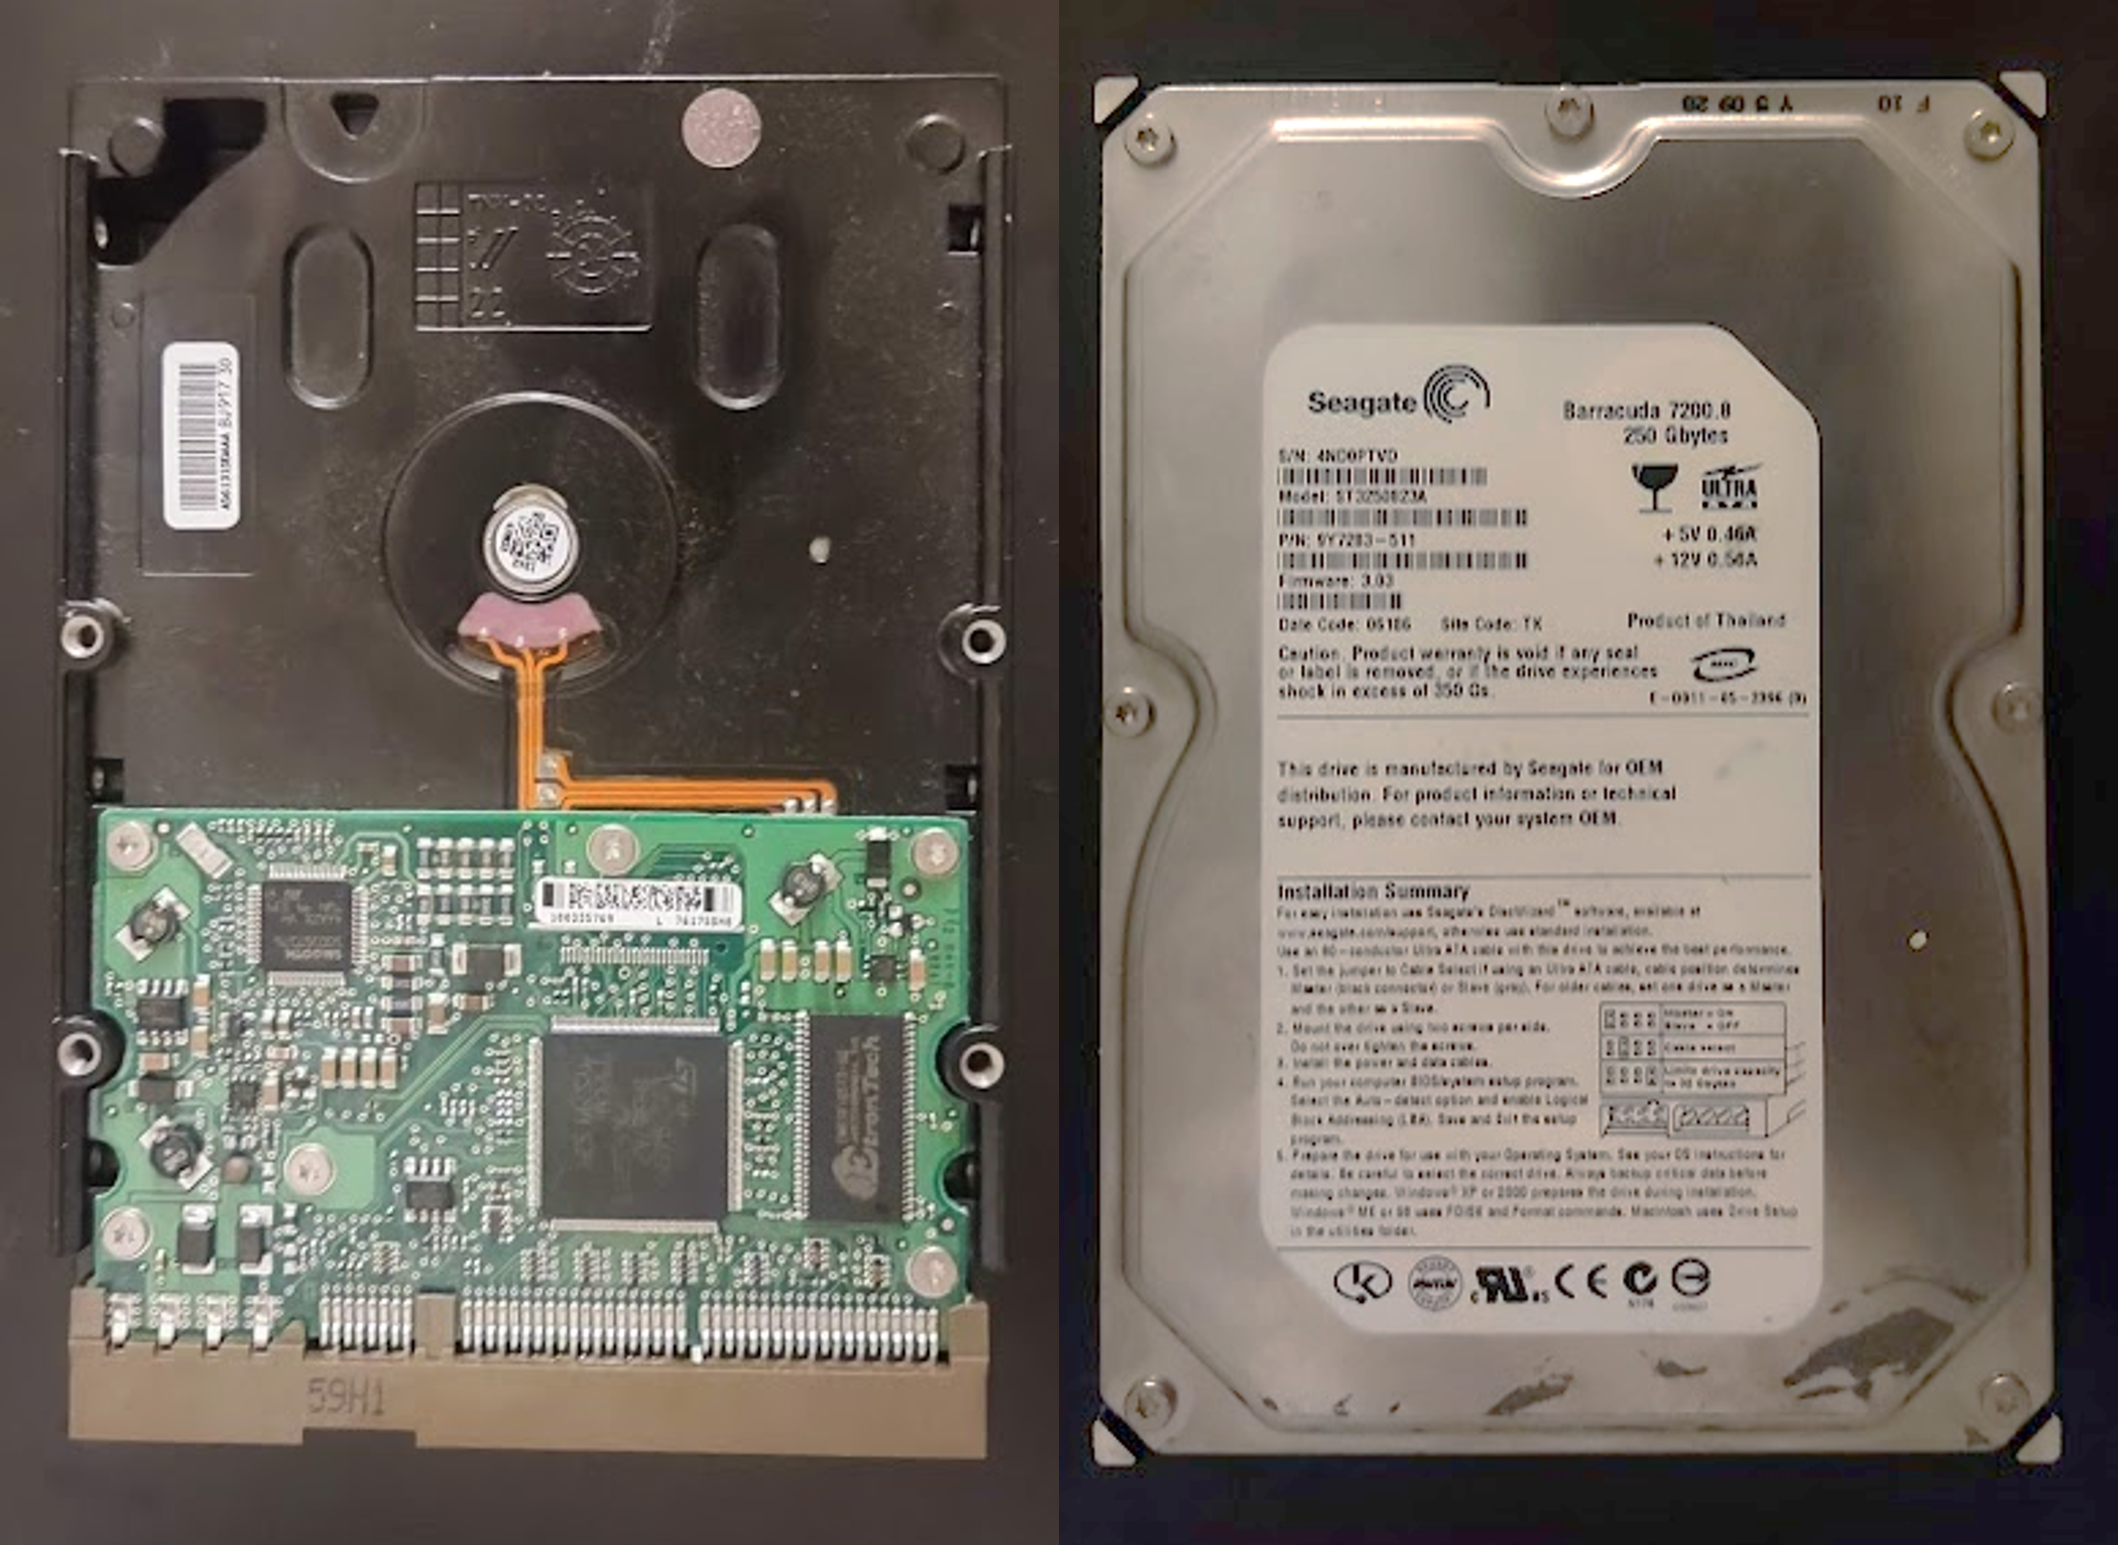
\includegraphics[scale=0.3]{../Images/disqueTIPEphoto.png}
            \end{center}
        \end{minipage}
        %
        \begin{minipage}{0.1\linewidth}
            \hfill
        \end{minipage}
        %
        \begin{minipage}{0.4\linewidth}
            \begin{center}
                \begin{tikzpicture}
                    \node[anchor=south west,inner sep=0] at (0.2,0.2) {\includesvg[width = 1.15\textwidth]{../Images/disque.svg}};
    
                    \draw[<->] (0, 2) --node[midway,above, sloped, align=center] {$\qty{146.9898}{\mm}$} (3, 3.75);
    
                    \draw[<->] (3.2, 3.8) --node[midway,above, sloped, align=center] {$\qty{101.6}{\mm}$} (5.3, 2.6);
    
                    \draw[<->] (5.5, 2.4) --node[midway,above, sloped, align=center] {$\qty{26.111}{\mm}$} (5.5, 1.6);
                \end{tikzpicture}
            \end{center}
        \end{minipage}
    }
\end{frame}

\begin{frame}[fragile]{Approche expérimentale}
    \begin{bash}
dd if=/dev/sda | hd | less
    \end{bash}

    \pause
    \begin{outputlog}
00000000  33 c0 fa 8e d8 8e d0 bc  00 7c 89 e6 06 57 8e c0  |3........|...W..|
00000010  fb fc bf 00 06 b9 00 01  f3 a5 ea 1f 06 00 00 52  |...............R|
00000020  52 b4 41 bb aa 55 31 c9  30 f6 f9 cd 13 72 13 81  |R.A..U1.0....r..|
00000030  fb 55 aa 75 0d d1 e9 73  09 66 c7 06 8d 06 b4 42  |.U.u...s.f.....B|
00000040  eb 15 5a b4 08 cd 13 83  e1 3f 51 0f b6 c6 40 f7  |..Z......?Q...@.|
00000050  e1 52 50 66 31 c0 66 99  e8 66 00 e8 35 01 4d 69  |.RPf1.f..f..5.Mi|
00000060  73 73 69 6e 67 20 6f 70  65 72 61 74 69 6e 67 20  |ssing operating |
00000070  73 79 73 74 65 6d 2e 0d  0a 66 60 66 31 d2 bb 00  |system...f`f1...|
00000080  7c 66 52 66 50 06 53 6a  01 6a 10 89 e6 66 f7 36  ||fRfP.Sj.j...f.6|
00000090  f4 7b c0 e4 06 88 e1 88  c5 92 f6 36 f8 7b 88 c6  |.{.........6.{..|
...
    \end{outputlog}\pause

    \begin{bash}
dd if=/dev/zero of=/dev/sda bs=32M
    \end{bash}

    \begin{outputlog}
00000000  00 00 00 00 00 00 00 00  00 00 00 00 00 00 00 00  |................|
*
f196b000
    \end{outputlog}

    \pause 
    \begin{itemize}
        \item Disque exposé pendant 8 semaines à Paris
    \end{itemize}
    
\end{frame}

\begin{frame}{Approche expérimentale}
    \begin{itemize}
        \item Disque \guill{trop grand}\pause

        \item Solutions de \guill{durcissement} déjà présentes\pause

        \item Matériel insuffisant\pause
    \end{itemize}

    Altitude insuffisante ($\qty{35}{\meter}$) ?
\end{frame}

\subsection{Données réelles}

\begin{frame}{Données réelles}
    \begin{minipage}{0.4\linewidth}
        \includegraphics[scale=0.4]{../Images/unscear2008cosmic.pdf}
    \end{minipage}
    %
    \begin{minipage}{0.1\linewidth}
        \hfill
    \end{minipage}\pause
    %
    \begin{minipage}{0.4\linewidth}
        \includegraphics[scale=0.5]{../Images/latitude.png}
    \end{minipage}
\end{frame}

\begin{frame}{Données réelles}
    \begin{bform}{\textsc{Ziegler} et \textsc{Lanford}, 1981}{}
        Un semi-conducteur de l'époque de $\qty{10}{\micro\meter\squared}$ est sujet à environ un \emph{soft-fail} par jour.
    \end{bform}
\end{frame}

\section{Solutions de durcissement}

\subsection{Durcissement matériel}

\begin{frame}{Durcissement matériel}
    \begin{minipage}{0.4\linewidth}
        \[ \mathrm{Al}_2\mathrm O_3\]

        \emph{Silicon On Sapphire (SOS)}
    \end{minipage}
    %
    \hfill\pause
    %
    \begin{minipage}{0.4\linewidth}
        \[ \mathrm{Si} O_2\]

        \emph{Silicon On Insulator (SOI)}
    \end{minipage}
\end{frame}

\begin{frame}{Durcissement matériel}
    \begin{itemize}
        \item SOS, SOI\pause
        
        \item Boîtiers résistants

        \item $\dots$\pause
    \end{itemize}

    Protection partielle
\end{frame}

\subsection{Durcissement logique : codes correcteurs}

\begin{frame}{Durcissement logique : codes correcteurs}
    \begin{itemize}
        \item Redondance \pause ($\dots$ optimisée)\pause

        \item \emph{Théorie des codes correcteurs}\pause
    \end{itemize}

    \begin{bdefinition}{Checksum}{}
        On appelle \hg{somme de contrôle} ou \hg{checksum} une information calculée à partir d'une donnée de plus grande taille, permettant de vérifier l'intégrité de cette donnée.
    \end{bdefinition}\pause

    \begin{itemize}
        \item Fonction de hachage, bit de parité, $\dots$
    \end{itemize}
\end{frame}

\begin{frame}{Code de \textsc{Hamming} $\p{7, 4}$}
    \[ \p{b_1, b_2, b_3, b_4} \xrightarrow[]{} (\underbrace{b_1, b_2, b_3, b_4}_{\text{message}},\ \underbrace{p_1, p_2, p_3}_{\text{contrôle}}) \]

    \begin{minipage}{0.4\linewidth}
        \begin{tikzpicture}
            \filldraw[color=main5, fill=main5!80, opacity=0.5, thick](1,2) circle (1.5);
            
            \filldraw[color=main1, fill=main1!80, opacity=0.5, thick](0,0) circle (1.5);

            \filldraw[color=main3, fill=main3!80, opacity=0.5, thick](2,0) circle (1.5);

            \node[main5!50!main1!50!black] at (0.2, 1.2) {$b_1$};
            \node[main5!50!main3!50!black] at (1.8, 1.2) {$b_2$};
            \node[main1!50!main3!50!black] at (1.05, 0) {$b_3$};

            \node[main1!50!main3!50!main5!50!black] at (1.05, 0.75) {$b_4$};

            \node[main5] at (1, 2.5) {$p_1$};

            \node[main1] at (-0.5, 0) {$p_2$};

            \node[main3] at (2.5, 0) {$p_3$};

            
        \end{tikzpicture}
    \end{minipage}
    %
    \qquad\pause
    \begin{minipage}{0.4\linewidth}
        \begin{NiceTabular}{|c||ccccccc|}[]
            \CodeBefore
                \rowcolor{main3!10}{1}
                \cellcolor{main21!40}{2-2,3-2,2-3,4-3,3-4,4-4,2-5,3-5,4-5,2-6,3-7,4-8}
                \cellcolor{main20!40}{4-2,3-3,2-4,3-6,4-6,2-7,4-7,2-8,3-8}
            \Body
                \toprule
                \text{ } & $b_1$ & $b_2$ & $b_3$ & $b_4$ & $p_1$ & $p_2$ & $p_3$ \\ \midrule
                $\color{main5}{\bigcdot}$ \\
                $\color{main1}{\bigcdot}$ \\
                $\color{main3}{\bigcdot}$ \\
                \bottomrule
        \end{NiceTabular}
    \end{minipage}
\end{frame}

\begin{frame}{Code de \textsc{Hamming} $\p{7, 4}$}
    \[ B = (\underbrace{b_1, b_2, b_3, b_4}_{\p{\bdZ/2\bdZ}^4}) \quad \xrightarrow{E = \bbG B} \quad \p{b_1, b_2, b_3, b_4, p_1, p_2, p_3} = E\]\pause

    \[ \bbG = \begin{pNiceMatrix}
        1 & 0 & 0 & 0\\
        0 & 1 & 0 & 0\\
        0 & 0 & 1 & 0\\
        0 & 0 & 0 & 1\\
        1 & 1 & 0 & 1\\
        1 & 0 & 1 & 1\\
        0 & 1 & 1 & 1\\
        \end{pNiceMatrix} \]

    
\end{frame}

\begin{frame}{Code de \textsc{Hamming} $\p{7, 4}$}
    \[ E = (\underbrace{b_1, b_2, b_3, b_4, p_1, p_2, p_3}_{\p{\bdZ/2\bdZ}^7}) \quad \xrightarrow{S = \bbH E} \quad \p{s_1, s_2, s_3} = S\]\pause

    \[ \bbH = \begin{pNiceMatrix}
        1 & 1 & 0 & 1 & 1 & 0 & 0\\
        1 & 0 & 1 & 1 & 0 & 1 & 0\\
        0 & 1 & 1 & 1 & 0 & 0 & 1
        \end{pNiceMatrix} \]\pause
    %
    \[ S = \bbH E = \p{0, 0, 0} \qquad \bbH \bbG = O_{3, 4}\]\pause
    %
    \[ \begin{array}{c}
        \bbH \p{E + e_i} = \bbH e_i = \p{s_1, s_2, s_3} \to \overline{s_1s_2s_3}^2\\
        e_1 \to 6\quad e_2 \to 5\quad e_3 \to 3\quad e_4 \to 7\quad e_5 \to 4 \quad e_6 \to 2\quad e_7 \to 1
    \end{array} \]\pause

    \[ E + 2 e_i = E\]
\end{frame}

\subsection{Durcissement logique : technologie RAID}

\begin{frame}{Durcissement logique : technologie RAID}
    \begin{center}
        \includegraphics[scale=0.3]{../Images/raid.png}
    \end{center}
\end{frame}

\begin{frame}{Durcissement logique : technologie RAID}
    \[ \p{\p{\bdZ/2\bdZ}^8, +} \qquad\pause 0 = \texttt{0x00} = \p{0, 0, 0, 0, 0, 0, 0, 0}\qquad\pause \p{\bdF_{2^8}, +, \times}\]\pause
    %
    \begin{itemize}
        \item $\times$ associatif, commutatif, distributif sur $+$\pause
    \end{itemize}

    \[ \forall n \in \bdF_{2^8}, \qquad \begin{cases}\p{n \times 2}_0 = n_7\\
        \p{n \times 2}_1 = n_0\\
        \p{n \times 2}_2 = n_1 + n_7\\
        \p{n \times 2}_3 = n_2 + n_7\\
        \p{n \times 2}_4 = n_3 + n_7\\
        \p{n \times 2}_5 = n_4\\
        \p{n \times 2}_6 = n_5\\
        \p{n \times 2}_7 = n_6
        \end{cases}\]

    \begin{itemize}
        \item $X^8 + X^4 + X^3 + X^2 + 1$, \qquad\pause $g = 2$ générateur de $\bdF_{256}$.
    \end{itemize}
\end{frame}

\begin{frame}{RAID-6}
    $n \geq 255$ disques
    %
    \[ p = u_0 + u_1 + \dots u_n = \sum_{k=0}^n u_k\]\pause
    %
    \[ q = g^0 \times u_0 + g^1 \times u_1 + \dots + g^{n-1} \times u_{n-1} = \sum_{k=0}^n g^k \times u_k\]\pause
    %
    \begin{itemize}
        \item $p$ et/ou $q \implies$ recalculer\pause

        \item $u_k \implies$ à partir de $p$\pause

        \item $u_k$ et $q \implies$ de même\pause

        \item $u_k$ et $p \implies$ \cf annexe.\pause

        \item $u_k$ et $u_\ell$ \cf annexe.\pause
    \end{itemize}

\end{frame}

\section{Annexes}

\begin{frame}[fragile]{Code de \textsc{Hamming}}

Matrice $\bbG$ :
    \begin{C}
const uint8_t g[7] =
        {
                0b1000,
                0b0100,
                0b0010,
                0b0001,
                0b1101,
                0b1011,
                0b0111
        };
    \end{C}
\end{frame}

\begin{frame}[fragile]{Code de \textsc{Hamming}}

Matrice $\bbH$ :
    \begin{C}
const uint8_t h[3] =
        {
            0b1101100,
            0b1011010,
            0b0111001
        };
    \end{C}
\end{frame}

\begin{frame}[fragile]{Code de \textsc{Hamming}}

Sommation des composantes dans $\p{\bdZ/2\bdZ}^8$:
    \begin{C}
uint8_t sumBits(uint8_t b)
{
    uint8_t s = 0;
    for (uint8_t m = 1; m < 0b10000000; m <<= 1) {
        if (b & m) s++;
    }
    return s & 0b0000001;
}
    \end{C}
\end{frame}

\begin{frame}[fragile]{Code de \textsc{Hamming}}

Multiplication par $\bbG$:
    \begin{C}
uint8_t hammingG(uint8_t b)
{
    uint8_t e = 0;
    for (uint8_t i = 0; i < 7; i++) {
        e <<= 1;
        if (sumBits(g[i] & b)) e |= 1;
    }
    return e;
}
    \end{C}
\end{frame}

\begin{frame}[fragile]{Code de \textsc{Hamming}}

Multiplication par $\bbH$:
    \begin{C}
uint8_t hammingH(uint8_t e)
{
    uint8_t s = 0;
    for (uint8_t i = 0; i < 3; i++)
    {
        s <<= 1;
        if (sumBits(h[i] & e)) s |= 1;
    }
    return s;
}
    \end{C}
\end{frame}

\begin{frame}[fragile]{Code de \textsc{Hamming}}

Correspondance avec $S$ et décodage avec correction d'une erreur :
    \begin{C}
const uint8_t sCor[8] =
        {
                0 << 0,
                1 << 0,
                1 << 1,
                1 << 4,
                1 << 2,
                1 << 5,
                1 << 6,
                1 << 3
        };

uint8_t hammingFix(uint8_t e) {
    return ((e ^ sCor[hammingH(e)]) & 0b1111000)
    >> 3;
}

    \end{C}
\end{frame}

\begin{frame}[fragile]{Test de performance}

    \begin{C}
int main() {
    uint8_t code = 0b1011;
    uint8_t pert = 1 << 4;
    int size = 10*1000*1000;
    time_t start = time(NULL);
    for (int i = 0; i < size; i++)
        if (hammingFix(hammingG(code) ^ pert)
        != code) {
            printf("Erreur d'éxécution !\n");
            return 1;
    }
    unsigned long d = difftime(time(NULL), start);
    printf("Exécution réussie en %ld s\n", d);
    return 0;
}
    \end{C}
    \begin{outputlog}
Exécution réussie en 1 s
    \end{outputlog}
\end{frame}

\begin{frame}{Calcul RAID-6 pour $u_i$ et $p$}
    \begin{align*}
        q &= \widetilde{q} + g^ku_k \\
        q + \widetilde{q} &= g^k u_k \\
        u_k &= \dfrac{q + \tilde{q}}{g^k}\\
        u_k &= \p{q + \widetilde q}\times g^{-k} \\
        u_k &= \p{q + \widetilde q}\times g^{255-k}
    \end{align*}
\end{frame}

\begin{frame}{Calcul RAID-6 pour $u_k$ et $u_\ell$}
    \[ \widetilde p + u_k + u_\ell = p \qquad\et\qquad \widetilde q + g^k u_k + g^\ell u_\ell = q\]

    \begin{align*}
        u_k &= \p{q + \widetilde q}\times g^{-k} + u_\ell \times g^{\ell -k}\\
        u_k &= \p{q + \widetilde q}\times g^{-k} + \p{p + \widetilde p + u_k} \times g^{\ell -k}\\
        u_k \times \p{g^{\ell - k} + 1} &= \p{q + \widetilde q}\times g^{-k} + \p{p + \widetilde p} \times g^{\ell -k}
    \end{align*}
    %
    Pour $x \neq y$ on a $g^{\ell - k} \neq 1$ d'où :
    %
    \[ u_k = \dfrac{\p{q + \widetilde q}\times g^{-k} + \p{p + \widetilde p} \times g^{\ell -k}}{g^{\ell - k} + 1}\]

\end{frame}

\begin{frame}[fragile]{RAID-6}
    \begin{C}
uint8_t tpow2(uint8_t u, int k)
{
    return (k >= 0) ? (u << k) : (u >> -k);
}
    \end{C}
\end{frame}

\begin{frame}[fragile]{RAID-6}
    \begin{C}
uint8_t computeP(const uint8_t *u, int n)
{
    uint8_t p = 0;
    for (int i = 0; i < n; i++) p ^= u[i];
    return p;
}

uint8_t computeQ(const uint8_t *u, int n)
{
    uint8_t q = 0;
    for (int i = 0; i < n; i++)
        q ^= tpow2(u[i], i);
    return q;
}
    \end{C}
\end{frame}

\begin{frame}[fragile]{RAID-6}
    \begin{C}
uint8_t computeUkFromP(uint8_t *u, int n,
    int k, int p)
{
    uint8_t ptilde = 0;
    for (int i = 0; i < n; i++)
        ptilde ^= (i != k) ? u[i] : 0;
    u[k] = p ^ ptilde;
    return u[k];
}
    \end{C}
\end{frame}

\begin{frame}[fragile]{RAID-6}
    \begin{C}
uint8_t computeUkFromQ(uint8_t *u, int n,
    int k, int q)
{
    uint8_t qtilde = 0;
    for (int i = 0; i < n; i++)
        qtilde ^= (i != k) ? tpow2(u[i], i) : 0;
    u[k] = tpow2(q ^ qtilde, -k);
    return u[k];
}
    \end{C}
\end{frame}

\begin{frame}[fragile]{RAID-6}
    \begin{C}
void computeUkUl(uint8_t *u, int n, int k,
    int l, int p, int q)
{
    uint8_t ptilde = 0;
    uint8_t qtilde = 0;
    for (int i = 0; i < n; i++) {
        if (i != k && i != l) {
            ptilde ^= u[i];
            qtilde ^= tpow2(u[i], i);
        }
    }
    u[l] = (tpow2(q ^ qtilde, -k) ^
        tpow2(p ^ ptilde, k - l ))
        / (tpow2(1, l - k) ^ 1);
    u[k] = (p ^ ptilde) ^ u[l];
}
    \end{C}
\end{frame}

\begin{frame}[fragile]{Test de performance}
    \begin{C}
int main()
{
    uint8_t* m = malloc(4 * sizeof(uint8_t));
    m[0] = 0b01;
    m[1] = 0b10;
    m[2] = 0b11;
    m[3] = 0b10;
    int size = 10*1000*1000;
    time_t start = time(NULL);
    for (int i = 0; i < size; i++) {
        uint8_t p = computeP(m, 4);
        uint8_t q = computeQ(m, 4);
        if (m[2] != computeUkFromP(m, 4, 2, p) ||
        m[2] != computeUkFromQ(m, 4, 2, q))
            return 1;
    \end{C}

\end{frame}

\begin{frame}[fragile]{Test de performance}
    \begin{C}
        computeUkUl(m, 4, 2, 3, p, q);
        if (m[2] != 0b11 || m[3] != 0b10)
            return 2;
    }
    unsigned long d = difftime(time(NULL), start);
    printf("Exécution réussie en %ld s", d);
    free(m);
    return 0;
}
    \end{C}
    \begin{outputlog}
        Exécution réussie en 2 s
    \end{outputlog}
\end{frame}


\section{Conclusion}

\end{document}